A partir dos conceitos de modelagem de agentes apresentados, foram elaboradas diversas metodologias para a concep��o e o desenvolvimento destes agentes. Em fun��o da sua utilidade em rela��o ao desenvolvimento de agentes \emph{BDI}, sem deixar de ser �til para qualquer outro tipo de sistema multiagente, bem como a abund�ncia de documenta��o e ferramentas de modelagem dispon�veis, a metodologia utilizada no decorrer deste trabalho � a chamada \emph{Prometheus} \cite{prometheus}.

A metodologia \emph{Prometheus} consiste de tr�s fases, descritas por \citeonline{prometheus} da seguinte forma:
\begin{itemize}
  \item Especifica��o de Sistema: � focada em identificar as funcionalidades b�sicas do sistema como um todo, tais como suas entradas (percep��es), sa�das (a��es), e quaisquer fontes importantes de dados compartilhados;
  \item Modelagem Arquitetural: utiliza as sa�das da fase anterior para determinar quais agentes o sistema conter� e como eles ir�o interagir;
  \item Modelagem Detalhada: � onde s�o especificados os componentes internos de cada agente e como tal agente realizar� suas tarefas dentro do sistema.
\end{itemize}

A figura 5 demonstra estas tr�s fases citadas acima de forma expl�cita, mostrando os artefatos gerados por cada fase, bem como os eventos que levam de uma fase a outra.

\begin{figure}[!htb]
	\centering
	\caption{Diagrama explicitando as fases da metodologia \emph{Prometheus}, obtido de \cite{prometheus}.}\label{fig:promehteus}
	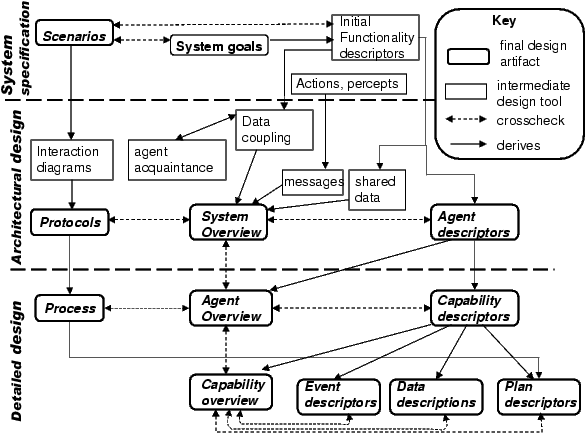
\includegraphics[width=1\textwidth]{figuras/prometheus.png}
\end{figure}

Vale notar que estas fases descritas acima e explicitadas na figura 5 constituem um processo iterativo de engenharia de software, e n�o um modelo de desenvolvimento do tipo cascata, sendo que estas fases n�o devem ser necessariamente executadas em alguma ordem em particular. \citeonline{prometheus} sugerem repetir o processo inteiro mais de uma vez, com um foco diferente a cada repeti��o, sendo que a primeira itera��o pode consistir inteiramente de atividades associadas a fase de especifica��o de sistema, itera��es subsequentes envolver�o uma mistura de atividades de fases diferentes, eventualmente com uma presen�a maior de atividades das fases seguintes.
